\documentclass[tikz=true]{standalone}
\usepackage{../main/NHQM}

\begin{document}
  

  \newcommand{\depth}{3}
  
  \pgfdeclareverticalshading{resonance}{100bp}
   {color(0bp)=(white); color(50bp)=(black!70); color(100bp)=(white)}
    
    %%%%%%%% HARMOSC NO LABELS
    
    \begin{tikzpicture}[
      domain=0:2,
      samples=200,
      ]
      \draw[->] (0, 0) -- (2, 0) node[above] {$r$};
      \draw[->] (0, -2.1) -- (0, 2) node[right] {$V$};
      \draw plot (\x, {\x*\x - 2});
      \clip (-2,-2.1) rectangle (2.1, 2.3);
    \end{tikzpicture}
    
    %%%%%%% HARMOSC LABELS
    
    \begin{tikzpicture}[
      domain=0:2,
      samples=200,
      ]
      \draw[->] (0, 0) -- (2, 0) node[above] {$r$};
      \draw[->] (0, -2.1) -- (0, 2) node[right] {$V$};
      \draw plot (\x, {\x*\x - 2});
      \foreach \y in {-1.3, -0.6, ..., 2} {
        \draw (0, \y) -- ($ ({ sqrt(\y + 2)} , \y) $);
        \draw[shorten >=0.5mm] (-1, 0)
          -- (0, \y);
      }
      \node[left, align=center, fill=white] 
        at (-0.2, 0)  {Bundna\\tillstånd};
      \clip (-2,-2.1) rectangle (2.1, 2.3);
    \end{tikzpicture}


    %%%%%% He5 NO LABELS
    
     \begin{tikzpicture}[
       domain=0:2.95,
       samples=200,
       ]
      \clip (-1.7,-2.1) rectangle (3.7,2.3);
       \draw[->] (0, 0) -- (3, 0) node[below] {$r$};
       \draw[->] (0, -2.1) -- (0, 2) node[right] {$V$};
       \draw plot (\x,{-2/(1 + exp((\x-1)/0.3))});
     \end{tikzpicture}
     
     
     %%%%%% He5 BOUND
     
     \begin{tikzpicture}[
       domain=0:2.95,
       samples=200,
       ]
      \clip (-1.7,-2.1) rectangle (3.7,2.3);
      
       \draw[->] (0, 0) -- (3, 0) node[below] {$r$};
       \draw[->] (0, -2.1) -- (0, 2) node[right] {$V$};
       \draw plot (\x,{-2/(1 + exp((\x-1)/0.3))});
       \foreach \x/\y in {1/-1, 1.33/-0.5} {
         \draw (0, \y)-- (\x, \y);
       }
       \node[left, align=center] 
         at (0,-0.75)  {Bundna\\tillstånd};
     \end{tikzpicture}
     
     
     %%%%%%% Spridda
     
     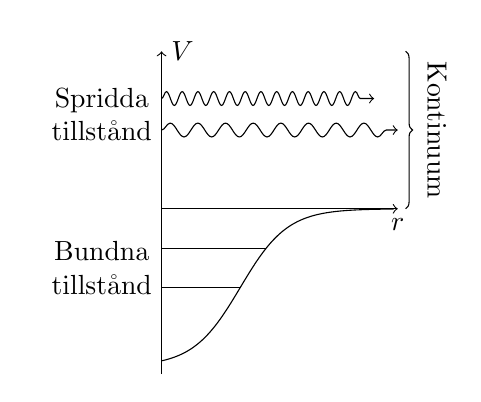
\begin{tikzpicture}[
       domain=0:2.95,
       samples=200,
       ]
      \clip (-1.7,-2.1) rectangle (3.7,2.3);
       \begin{scope}[->]
         \draw[decorate, decoration={snake, post length=1mm}] 
           (0, 1) -- (3, 1);
         \draw[decorate, decoration={snake, post length=1mm,
                                     segment length = 2mm}] 
           (0, 1.4) -- (2.7, 1.4);
       \end{scope}
       
       \begin{scope}[left, fill=white, align=center]
         \node at (0, 1.2) {Spridda\\tillstånd};
       \end{scope}
      
       \draw[->] (0, 0) -- (3, 0) node[below] {$r$};
       \draw[->] (0, -2.1) -- (0, 2) node[right] {$V$};
       \draw plot (\x,{-2/(1 + exp((\x-1)/0.3))});
       \foreach \x/\y in {1/-1, 1.33/-0.5} {
         \draw (0, \y)-- (\x, \y);
       }
       \node[left, align=center] 
         at (0,-0.75)  {Bundna\\tillstånd};
         
         
       \draw[decorate, decoration={brace}] 
         (3.1,2) -- +(0,-2) node[midway, xshift=0.4cm, rotate=-90] {Kontinuum};
     \end{tikzpicture}
    
      
    \begin{tikzpicture}[
      domain=0:2.95,
      samples=200,
      ]
      \clip (-1.7,-2.1) rectangle (3.7,2.3);
      \begin{scope}[->]
        \draw[decorate, decoration={snake, post length=1mm}] 
          (0, 1) -- (3, 1);
        \draw[decorate, decoration={snake, post length=1mm,
                                    segment length = 2mm}] 
          (0, 1.4) -- (2.7, 1.4);
      \end{scope}
      
      \shade[shading=resonance]
        (0,0.5) ++ (0,-0.02) rectangle +(3,0.04);
      \begin{scope}[left, fill=white, align=center]
        \node at (0, 1.2) {Spridda\\tillstånd};
        \node at (0, 0.5) {Resonans};
      \end{scope}
     
      \draw[->] (0, 0) -- (3, 0) node[below] {$r$};
      \draw[->] (0, -2.1) -- (0, 2) node[right] {$V$};
      \draw plot (\x,{-2/(1 + exp((\x-1)/0.3))});
      \foreach \x/\y in {1/-1, 1.33/-0.5} {
        \draw (0, \y)-- (\x, \y);
      }
      \node[left, align=center] 
        at (0,-0.75)  {Bundna\\tillstånd};
        
        
      \draw[decorate, decoration={brace}] 
        (3.1,2) -- +(0,-2) node[midway, xshift=0.4cm, rotate=-90] {Kontinuum};
    \end{tikzpicture}
\end{document}